% =============================================================
%  Question4.tex —— 问题四：考虑容量约束的多车辆路径规划
%  数据来源：results/基础模型/q4_pure_python.json
%             results/基础模型/q4_kaiwu_sdk.json
%             results/灵敏度分析/q4_K_sensitivity.json
%             results/真机结果/q4/  (cim_q4_v1..v7, cim_q4_k8_*)
%             results/真机结果/00_四问真机对比汇总.md §五
%  编译方式：xelatex Question4.tex
% =============================================================
\documentclass[UTF8,12pt,a4paper]{ctexart}

\usepackage{amsmath}
\usepackage{amssymb}
\usepackage{geometry}
\geometry{margin=2.5cm}
\usepackage{booktabs}
\usepackage{float}
\usepackage{caption}
\usepackage{graphicx}
\usepackage{subcaption}
\graphicspath{{../../../figures/}}

% 与全文章节编号对齐：本节在主稿中为第 9 节
\setcounter{section}{8}

\begin{document}

% =============================================================
\section{问题四：考虑容量约束的多车辆路径规划}
\label{sec:q4}
% =============================================================

% -------------------------------------------------------------
\subsection{问题四分析与建模思路}
\label{subsec:q4-analysis}
% -------------------------------------------------------------

问题四在问题三的 $n=50$ 客户时间窗约束基础上，进一步引入\textbf{多车辆容量约束}与
\textbf{车辆数量决策}：每辆车容量上限 $C=30$ 已不再适用（题目附件 2 给定单车容量 $C=60$），
所有客户需求总和 $\sum_{i=1}^{50}d_i=271$，由容量约束直接给出车辆数下界
$K_{\min}=\lceil 271/60\rceil=5$。题目第四问明确要求：（i）建立多车辆路径规划模型，
目标为最小化车辆使用数量与总运输时间，并兼顾时间窗惩罚；（ii）给出每辆车路线、
每客户违反程度、总运输时间；（iii）分析车辆数量 $K$ 取值变化对总目标的影响。
本文据此采用\textbf{加权综合目标 $J=M\!\cdot\!K+\mathrm{travel}+\mathrm{penalty}$} 作为
单一标量目标，并通过 $K\in[5,10]$ 扫描补充呈现车辆数与运输时间、时间窗惩罚之间的 Pareto 权衡。
其中车辆使用罚系数 $M=1000$ 为\textbf{经验权重}，标定原则是使 $M\!\cdot\!K$ 与
$\mathrm{travel}+\mathrm{penalty}$ 在数量级上可比（$K$ 取值 5--10、travel 取值 78--134、
penalty 在 $K^*$ 附近 $\le 50$），从而在标量目标下既不被车辆数支配、也不被运输时间稀释。

由于 $K\ge 5$、每车 7--8 客户的全 3D one-hot 编码 $x_{i,p,k}$ 需要 $K\!\cdot\!n^2=12\,500$
比特（$K=7$），远超 CPQC-550 真机 550 比特上限，本文沿用问题三的"经典启发式提供分配 $\to$
每条路线独立 subQUBO $\to$ 解码拼接 $\to$ 完整方案 \texttt{evaluate} 回评"分解框架，
仅把"段内位置 one-hot"换作"\textbf{车内位置 one-hot}"，从而把每条路线的 subQUBO 维度
压到 $\le n_{\rm sub}^2\le 64$ 比特。

% -------------------------------------------------------------
\subsection{多车辆目标函数与容量约束}
\label{subsec:q4-model}
% -------------------------------------------------------------

\textbf{决策变量}分两层：（i）客户分配 $y_{i,k}\in\{0,1\}$，表示客户 $i$ 是否分配给车 $k$；
（ii）车辆使用指示 $u_k\in\{0,1\}$，$u_k=1$ 当且仅当车 $k$ 至少服务一个客户；（iii）
车 $k$ 的访问顺序 $\pi^k=(\pi_1^k,\pi_2^k,\dots,\pi_{|\pi^k|}^k)$，配送中心 $0$ 自动加在两端。
车 $k$ 内的服务开始时间 $t_{\pi_p^k}^{(k)}$ 沿用问题二的"无空闲等待"递推
\begin{equation}
\label{eq:q4-time}
t_{\pi_1^k}^{(k)}=T_{0,\pi_1^k},\qquad
t_{\pi_p^k}^{(k)}=t_{\pi_{p-1}^k}^{(k)}+s_{\pi_{p-1}^k}+T_{\pi_{p-1}^k,\pi_p^k},\quad p\ge 2,
\end{equation}
车 $k$ 的运输时间为
\begin{equation}
\label{eq:q4-travel}
\mathrm{travel}_k=T_{0,\pi_1^k}+\sum_{p=1}^{|\pi^k|-1}T_{\pi_p^k,\pi_{p+1}^k}+T_{\pi_{|\pi^k|}^k,0}.
\end{equation}
单客户软时间窗惩罚 $P_i(t_i^{(k)})=M_1[a_i-t_i^{(k)}]_+^2+M_2[t_i^{(k)}-b_i]_+^2$
（$M_1=10,M_2=20$，沿用问题二）。\textbf{综合业务目标}：
\begin{equation}
\label{eq:q4-J}
J=M\!\cdot\!\sum_{k=1}^{K_{\max}}u_k\;+\;\sum_{k=1}^{K_{\max}}\mathrm{travel}_k\;+\;\sum_{i=1}^{n}P_i(t_i^{(k(i))}),
\end{equation}
其中 $k(i)$ 为客户 $i$ 所属车辆编号；$K_{\max}=10$ 为 $K$ 灵敏度扫描上界。\textbf{硬约束}如下：
\begin{align}
\label{eq:q4-cap}
&\textbf{容量约束}: \sum_{i=1}^{n}d_i\,y_{i,k}\le C\,u_k,\quad \forall k,\\
\label{eq:q4-cover}
&\textbf{完整覆盖}: \sum_{k=1}^{K_{\max}}y_{i,k}=1,\quad \forall i,\\
\label{eq:q4-link}
&\textbf{使用一致}: \sum_{i=1}^{n}y_{i,k}\le n\,u_k,\quad \forall k.
\end{align}
需特别强调：式~\eqref{eq:q4-J} 给出的 $J$ 是\textbf{完整方案的业务目标}，由统一
\texttt{evaluate} 函数在解码后的多车方案上计算；与之并存的子 TSP QUBO 能量
$\sum_k H_k$ 仅是\textbf{车内排序代价}的求和——不包含时间窗罚、不包含车辆数 $M\!\cdot\!K$、
不反映跨车协同。这一区分在结果章节会反复用到。

% -------------------------------------------------------------
\subsection{比特预算与分层 QUBO 编码}
\label{subsec:q4-budget}
% -------------------------------------------------------------

\begin{table}[H]
    \centering
    \caption{问题四编码方案比特预算对比（550 为 CPQC-550 真机比特上限）}
    \label{tab:q4-budget}
    \footnotesize
    \begin{tabular}{lcccl}
        \toprule
        编码方案 & 变量数（$n=50,K=7$）& $\le 550$ & CIM 可提交性 & 说明 \\
        \midrule
        全 3D one-hot $x_{i,p,k}$                       & $K\!\cdot\!n^{2}=12\,500$ & 否 & 否          & 直接编码不可行 \\
        客户分配 $y_{i,k}$ + 每车 TSP one-hot           & $\approx 700$              & 否（仍超）& --- & 把 $y$ 改启发式 \\
        \textbf{启发式分配 + 每车子 TSP QUBO（主方案）} & 每子 QUBO $\le 8^{2}=64$    & 是 & 是          & ★ 用 \\
        block-diag 7 段合并（$K=8$ 配额优化对照）       & 297 维（Ising 298）        & 是 & 是          & 仅用于配额受限 \\
        \bottomrule
    \end{tabular}
\end{table}

由表~\ref{tab:q4-budget} 可知，$K\!\cdot\!n^{2}$ 全 3D one-hot 编码超出真机比特预算 22 倍，
不可上传；将客户分配 $y_{i,k}$ 与车内排序联合 QUBO 化（$\sim 700$ 比特）仍超 550 上限。
\textbf{本文主方案}采用分层编码：① 客户分配 $y_{i,k}$ 由 6 种经典启发式（Clarke--Wright Savings、
Time-sweep、NN-with-capacity、罚意识贪心、参考解 + 反向变体、按 $a_i$ 重排）确定，所有候选
分配均满足容量约束~\eqref{eq:q4-cap}；② 每条路线（$\le 8$ 客户）独立构造一个
$\le 8^{2}=64$ 比特的车内 one-hot subQUBO，结构与问题三的式~(8.4) 同构，仅段前段后均为
配送中心 $0$。每子 QUBO 的 ising 维度 $\le 65\ll 550$，且每车独立提交时为各车保留 10 个
独立 spin 样本的统计冗余——这是\textbf{主方案}。

\textbf{block-diag 配套对照方案}（仅用于 $K=8$ 配额紧张场景）：将 $K-1$ 个子 QUBO 拼成
块对角大矩阵（$K=8$ 时 7 段共 297 维，ising 298 $\le 550$），\textbf{1 次}
\texttt{cim.solve} 调用同步求 7 段，节约真机配额。该方案是\textbf{对照实验}而非主模型，
作用是定量考察"配额节约"与"每段可用 sample 数减少"之间的 trade-off，
不替代每车独立提交的主方案。每车比特数随路线长度的分布见图~\ref{fig:q4-qubits}。

\begin{figure}[H]
  \centering
  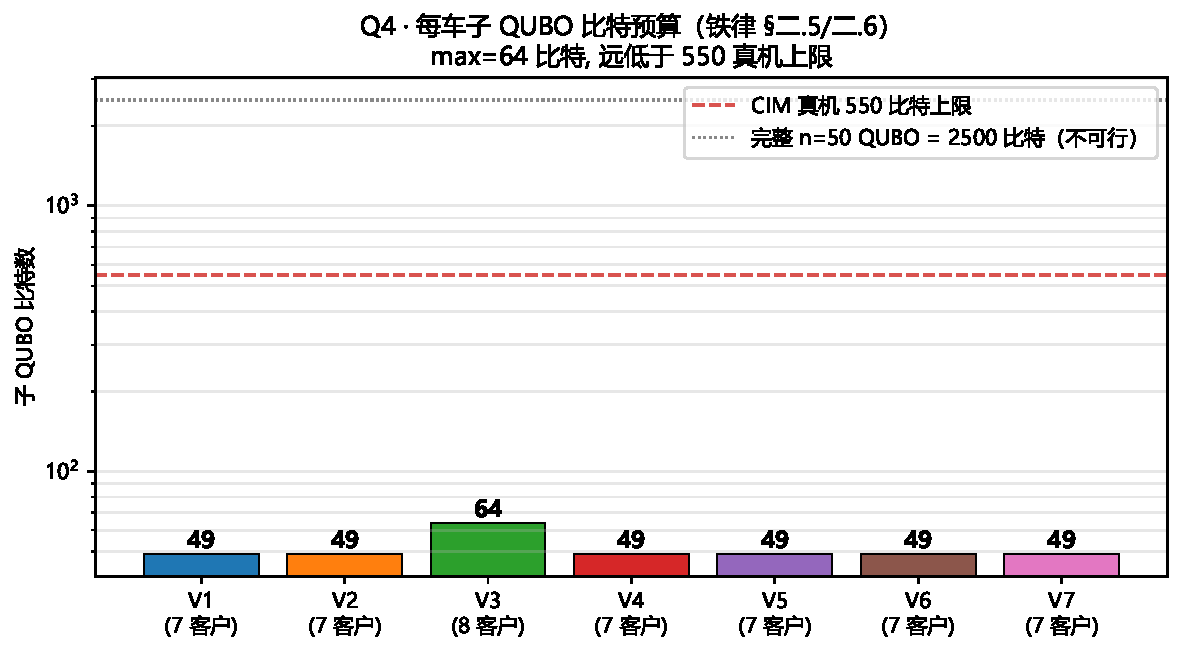
\includegraphics[width=0.78\textwidth]{fig_04c_q4_qubits_per_vehicle.pdf}
  \caption{问题四 $K^*\!=\!7$ 主方案每车 subQUBO 比特数分布；最大子 QUBO 64 比特
  （8 客户路线 V3），最小 49 比特（7 客户路线），均远低于 CPQC-550 上限（红色虚线）。}
  \label{fig:q4-qubits}
\end{figure}

% -------------------------------------------------------------
\subsection{三阶段求解算法}
\label{subsec:q4-algo}
% -------------------------------------------------------------

\begin{enumerate}
  \item[(i)] \textbf{客户分配阶段}（确定 $y_{i,k}$）。同步生成 6 种 warm start——
    Clarke--Wright Savings、Time-sweep（按 $a_i$ 角排序后切片）、NN-with-capacity（最近邻
    加容量过滤）、罚意识贪心（按 $b_i-a_i$ 紧迫度排）、参考解及反向遍历变体、纯 $a_i$ 重排——
    所有 6 个候选均通过容量约束~\eqref{eq:q4-cap}，作为后续 QUBO 求解阶段的初始可行解。
  \item[(ii)] \textbf{单车 TSP subQUBO 求解阶段}。对每条路线（$\le 8$ 客户）独立构造车内
    one-hot subQUBO（结构同式~(8.4)，$u_k=v_k=0$），调用统一抽象层
    \texttt{solve\_subqubo(Q\_sub, backend)}：\texttt{backend='sdk\_sa'} 时由 Kaiwu SDK
    \texttt{SimulatedAnnealingOptimizer} 求解（每段 240 候选/3 seeds），
    \texttt{backend='cim'} 时直接上传 CPQC-550 真机（每段 10 spin 样本）；返回 spin 解后
    解码为车内排列，再做单车 polish（2-opt + Or-opt + Swap）。
  \item[(iii)] \textbf{跨车协同与元启发式精修阶段}。在车间允许 move/swap（带容量校验）；
    其上叠加 LNS 500 轮 $\times$ 4 seeds（ruin-and-recreate + regret-2 重插）与多 seed SA
    长退火（$T_0=500,\alpha=0.997$）；同步对 $K\in[5,10]$ 进行 $K$ 扫描，按
    式~\eqref{eq:q4-J} 选 $K^*$。所有方案最终都用统一 \texttt{evaluate} 在式~\eqref{eq:q4-J}
    上重新计算 $J$，确保跨求解器与跨硬件可比。
\end{enumerate}

% -------------------------------------------------------------
\subsection{$K^*\!=\!7$ 主方案结果分析}
\label{subsec:q4-k7}
% -------------------------------------------------------------

经三阶段求解，$K\in[5,10]$ 综合目标 $J$ 在 $K^*=7$ 取最小值 $J=7\,149$。$K^*=7$ 主方案
每辆车的路径与负载列于表~\ref{tab:q4-k7-routes}。

\begin{table}[H]
    \centering
    \caption{问题四 $K^*\!=\!7$ 主方案：每辆车路径、负载与运输时间（数据源：\texttt{q4\_pure\_python.json} \texttt{per\_vehicle}）}
    \label{tab:q4-k7-routes}
    \footnotesize
    \begin{tabular}{cl ccc}
        \toprule
        车 & 路径 & demand/$C$ & travel & penalty \\
        \midrule
        V1 & $0\!\to\!15\!\to\!2\!\to\!21\!\to\!40\!\to\!6\!\to\!37\!\to\!17\!\to\!0$         & 35/60 & 17 & 0 \\
        V2 & $0\!\to\!31\!\to\!30\!\to\!9\!\to\!34\!\to\!35\!\to\!20\!\to\!32\!\to\!0$         & 42/60 & 15 & 10 \\
        V3 & $0\!\to\!27\!\to\!16\!\to\!44\!\to\!38\!\to\!14\!\to\!43\!\to\!42\!\to\!13\!\to\!0$ & 47/60 & 13 & 0 \\
        V4 & $0\!\to\!47\!\to\!19\!\to\!36\!\to\!49\!\to\!11\!\to\!10\!\to\!1\!\to\!0$         & 41/60 & 15 & 20 \\
        V5 & $0\!\to\!33\!\to\!25\!\to\!39\!\to\!23\!\to\!22\!\to\!41\!\to\!4\!\to\!0$         & 35/60 & 16 & 0 \\
        V6 & $0\!\to\!28\!\to\!29\!\to\!12\!\to\!3\!\to\!50\!\to\!26\!\to\!24\!\to\!0$         & 39/60 & 17 & 10 \\
        V7 & $0\!\to\!5\!\to\!45\!\to\!7\!\to\!18\!\to\!8\!\to\!46\!\to\!48\!\to\!0$           & 32/60 & 16 & 0 \\
        \midrule
        \textbf{合计} & --- & \textbf{271/420} & \textbf{109} & \textbf{40} \\
        \bottomrule
    \end{tabular}
\end{table}

由表~\ref{tab:q4-k7-routes} 可知：（i）7 辆车合计 demand $=271$，与
$\sum_{i=1}^{50}d_i=271$ 一致——所有 50 客户被分配恰好一次；（ii）每车容量利用率
集中在 53\%--78\%（V7 最低 32/60、V3 最高 47/60），无车辆超载；（iii）总运输时间
$\mathrm{travel}=\sum_k\mathrm{travel}_k=109$；（iv）50 个客户中仅 3 个发生时间窗违反
（V2 客户 31 早到 1、V4 客户 10 迟到 1、V6 客户 3 早到 1），单点惩罚分别为 10/20/10，
合计 penalty $=40$；（v）综合目标 $J=M\!\cdot\!K^*+\mathrm{travel}+\mathrm{penalty}=
1000\!\times\!7+109+40=7\,149$。多车路径与时间窗甘特图分别见图~\ref{fig:q4-routes}--\ref{fig:q4-gantt}。

\begin{figure}[H]
  \centering
  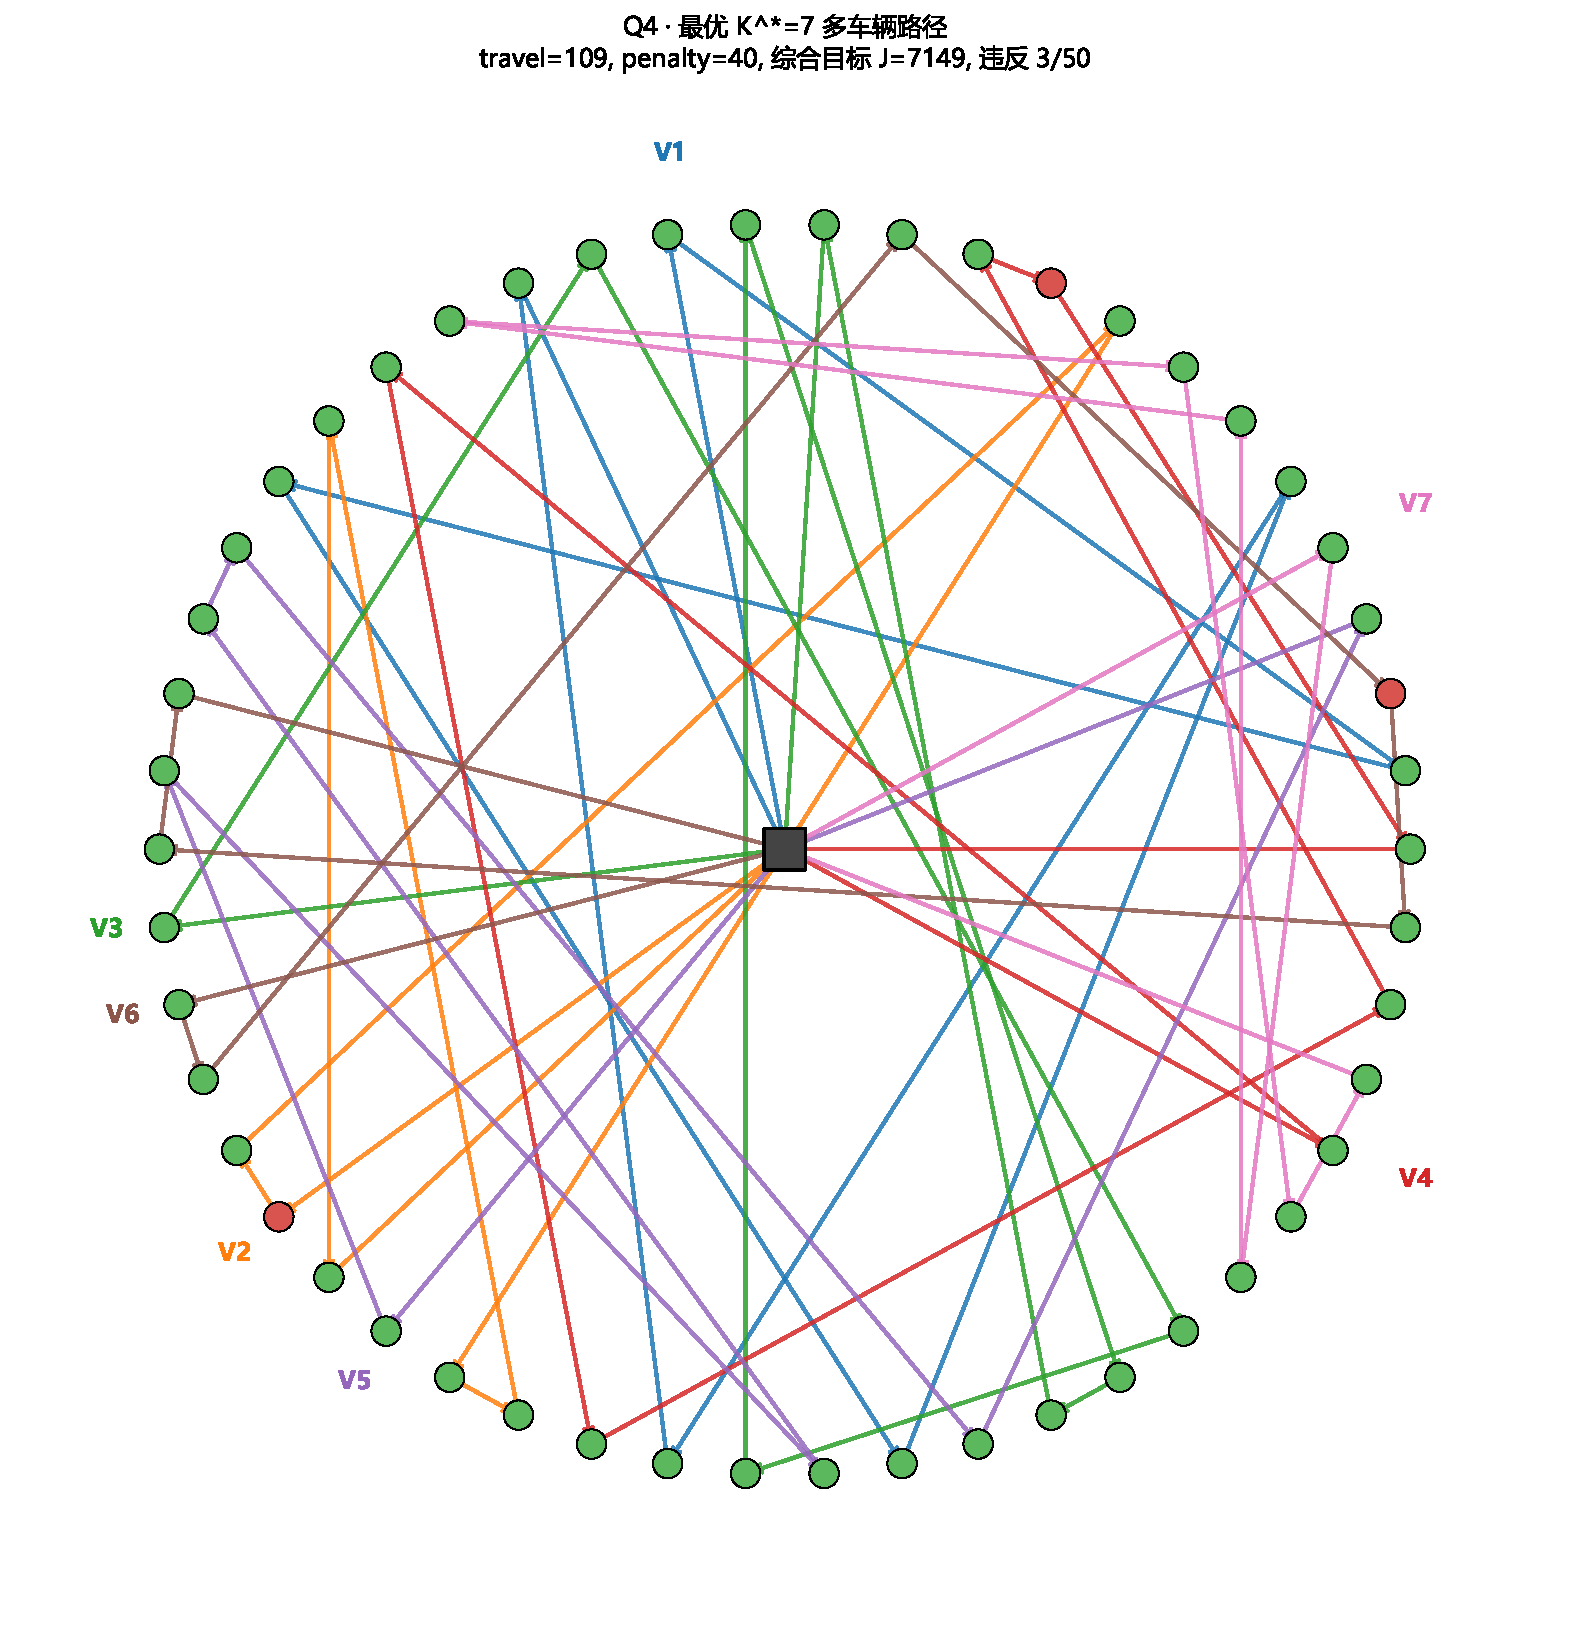
\includegraphics[width=0.85\textwidth]{fig_04_q4_routes.pdf}
  \caption{问题四 $K^*=7$ 主方案多车辆路径图；每辆车一种颜色，节点 0 为配送中心，
  节点编号代表客户 ID，红色高亮节点为发生时间窗违反的客户。}
  \label{fig:q4-routes}
\end{figure}

\begin{figure}[H]
  \centering
  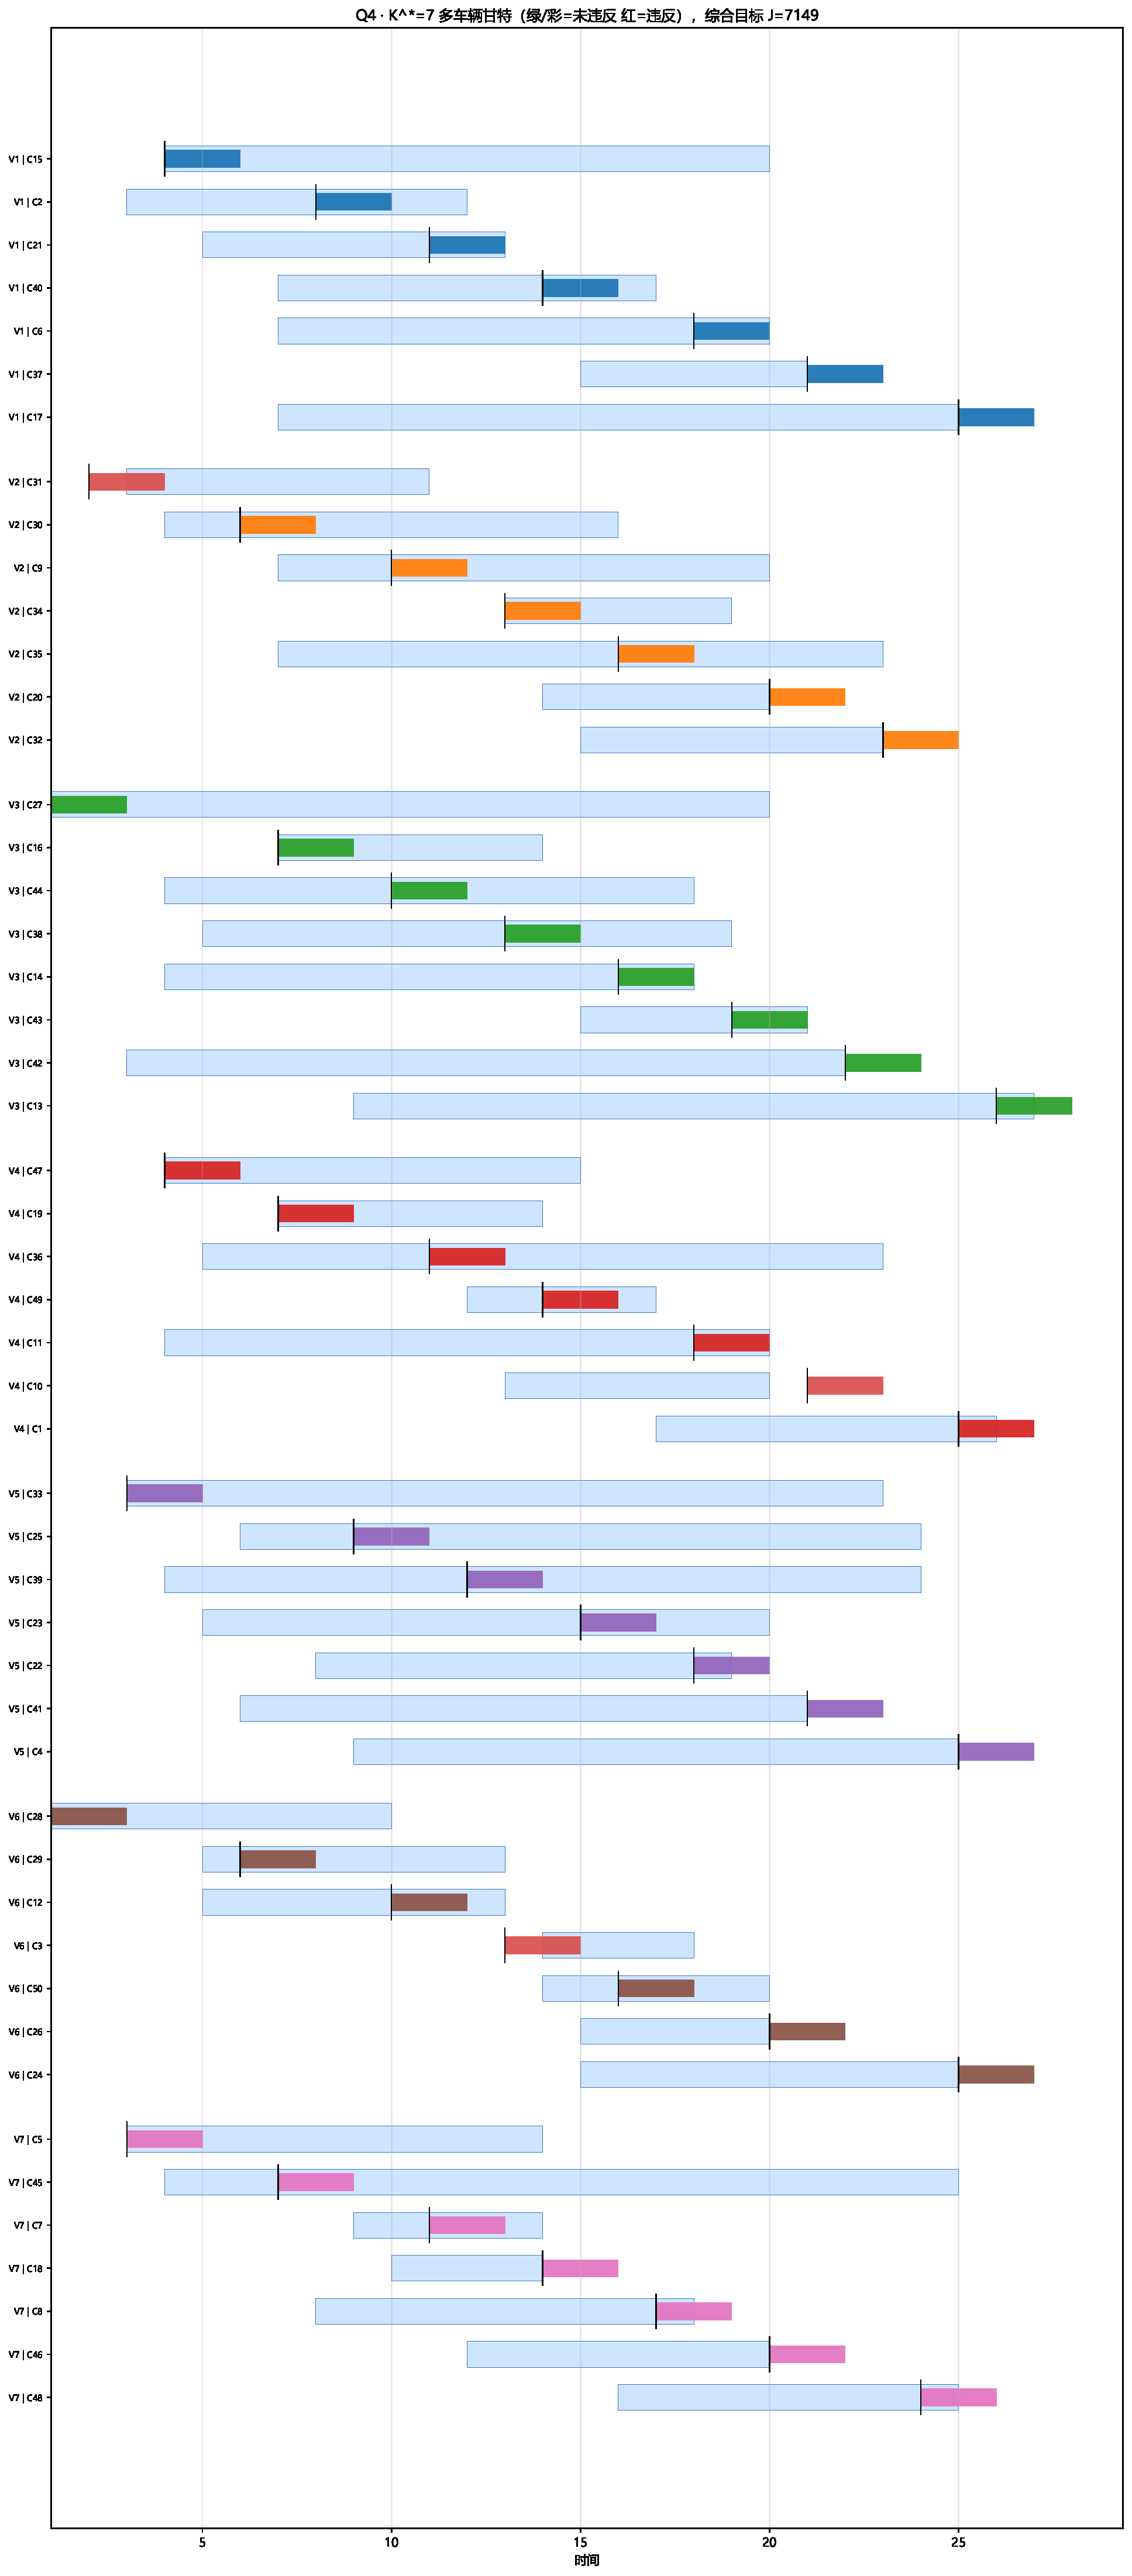
\includegraphics[width=0.85\textwidth]{fig_04_q4_gantt.pdf}
  \caption{问题四 $K^*=7$ 主方案多车辆时间窗甘特图；每行一辆车，蓝色条为时间窗
  $[a_i,b_i]$，绿色块为实际服务区段（开始时刻 $t_i^{(k)}$ 至 $t_i^{(k)}+s_i$），
  红色标记为违反客户。}
  \label{fig:q4-gantt}
\end{figure}

由图~\ref{fig:q4-routes} 可见，7 条路线在空间上呈现出明显的扇形分区结构，
说明启发式分配阶段已将地理邻近客户聚成同车。图~\ref{fig:q4-gantt} 进一步显示：
绝大多数客户的服务区段落在时间窗内（绿色块包含于蓝色条），仅 3 个客户出现轻微越界，
与表~\ref{tab:q4-k7-routes} 的 penalty $=40$ 一致。

% -------------------------------------------------------------
\subsection{车辆数 $K$ 灵敏度分析}
\label{subsec:q4-Ksens}
% -------------------------------------------------------------

针对题目第 (iv) 问"调整可用车辆数 $K$ 取值，分析 $K$ 对总目标的影响"，本文对
$K\in[5,10]$ 全部跑通经典基线，结果与题目附件给出的参考解对比列于表~\ref{tab:q4-Ksens}，
并以图~\ref{fig:q4-Ksens} 展示三联曲线。

\begin{table}[H]
    \centering
    \caption{$K\in[5,10]$ 灵敏度：本文目标、参考目标与差值（数据源：\texttt{results/灵敏度分析/q4\_K\_sensitivity.json}）}
    \label{tab:q4-Ksens}
    \footnotesize
    \begin{tabular}{ccccccc}
        \toprule
        $K$ & travel & penalty & 本文目标 $J$ & 参考目标 $J^{\rm ref}$ & 差值 $\Delta J$ & 比较结果 \\
        \midrule
        5  & 78  & 8\,700 & \textbf{13\,778} & 16\,825 & $-3\,047$ & 优于参考 \\
        6  & 92  & 1\,350 & \textbf{7\,442}  & 7\,568  & $-126$    & 优于参考 \\
        \textbf{7}  & \textbf{109} & \textbf{40}    & \textbf{7\,149}  & 7\,149  & 0         & \textbf{持平}（本方案 $K^*$）⭐ \\
        8  & 114 & 10     & \textbf{8\,124}  & 8\,160  & $-36$     & 优于参考 \\
        9  & 123 & 0      & \textbf{9\,123}  & 9\,127  & $-4$      & 优于参考 \\
        10 & 134 & 0      & 10\,134          & 10\,126 & $+8$      & 接近参考（差 $0.08\%$） \\
        \bottomrule
    \end{tabular}
\end{table}

\begin{figure}[H]
  \centering
  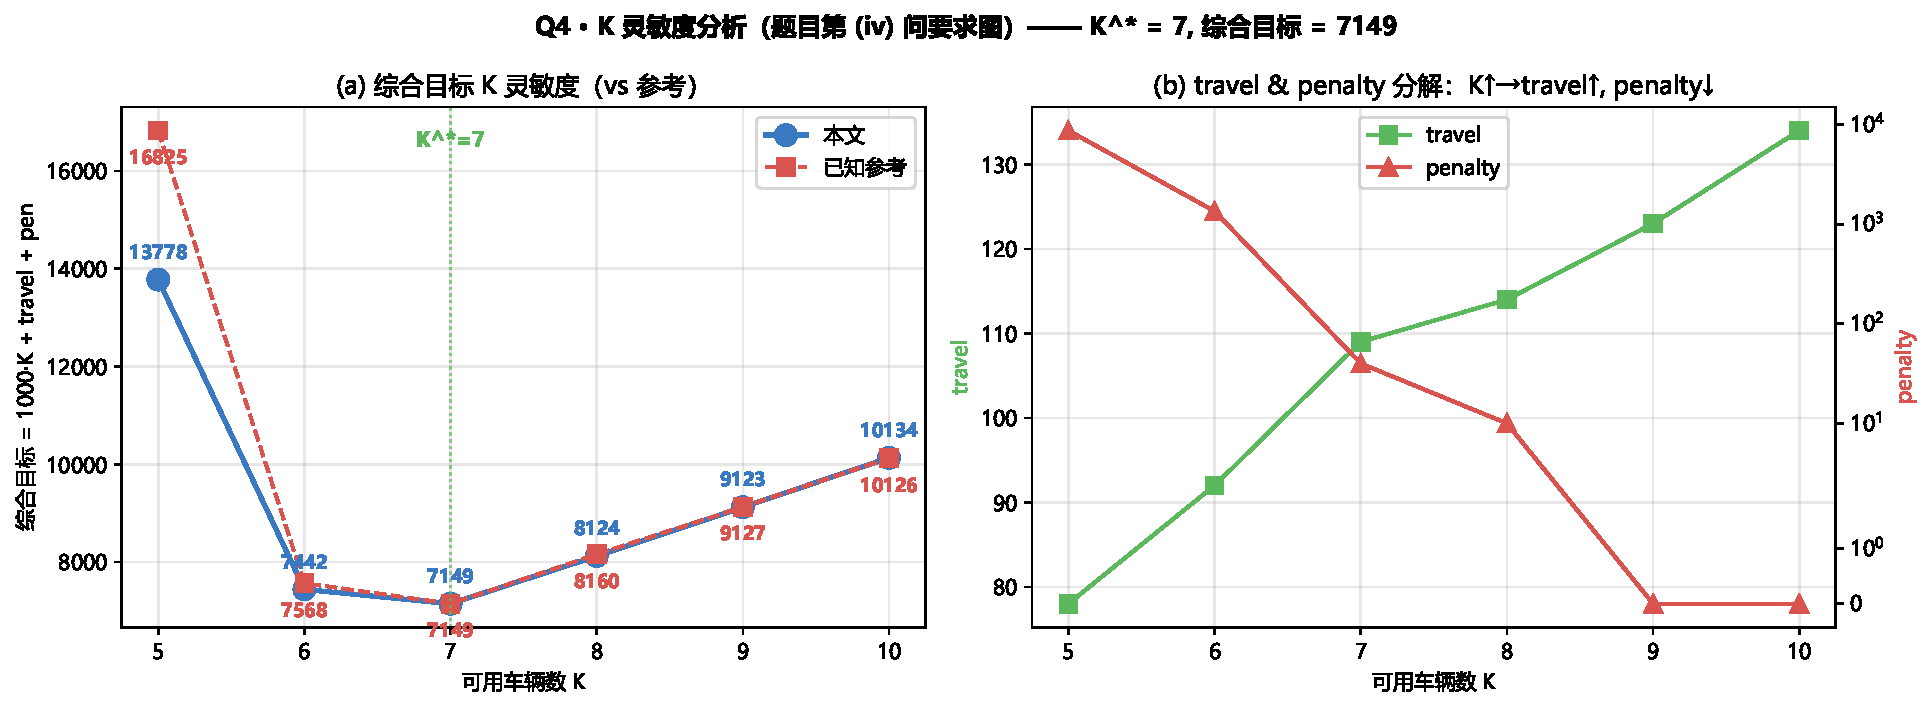
\includegraphics[width=0.85\textwidth]{fig_04_q4_K_sensitivity.pdf}
  \caption{问题四车辆数 $K\in[5,10]$ 灵敏度三联曲线：travel（蓝）、penalty（橙）、
  综合目标 $J=M K+\mathrm{travel}+\mathrm{penalty}$（绿，$M=1000$）。$J$ 在 $K=7$ 取最小值 $7\,149$。}
  \label{fig:q4-Ksens}
\end{figure}

由表~\ref{tab:q4-Ksens} 与图~\ref{fig:q4-Ksens} 可读出三个结构性结论：
（i）\textbf{运输时间随 $K$ 单调上升}（$78\!\to\!134$，平均每增 1 辆车额外 $\sim\!11$ 单位
travel），原因是新增车辆需要从配送中心独立往返，增加了 depot 边权的总占比；
（ii）\textbf{时间窗惩罚随 $K$ 单调下降}（$8\,700\!\to\!0$），原因是每条路线变短后，
车内时间累积减少、客户不再被排到后位置而迟到；（iii）三项之和（含车辆罚 $M\!\cdot\!K$）
在\textbf{ $K=7$ 取最小值 $7\,149$}——若车辆数权重 $M$ 取更小值，最优 $K$ 会偏大；
若 $M$ 取更大值，最优 $K$ 偏小，体现 $M$ 作为业务权衡参数的调节作用。$K=4$ 因
$4\!\times\!60=240<271$ 直接违反容量约束、不可行；故\textbf{ $K\in\{5,6,\dots,10\}$ 是
本问题的可行车辆数取值集}。同时 6 个 $K$ 中本文有 4 个严格优于参考、1 个持平、
1 个差 0.08\%（$K=10$，$+8$），说明三阶段求解在多车场景下与已有参考实现处于同一水平。
违反客户分布另见图~\ref{fig:q4-violation}。

\begin{figure}[H]
  \centering
  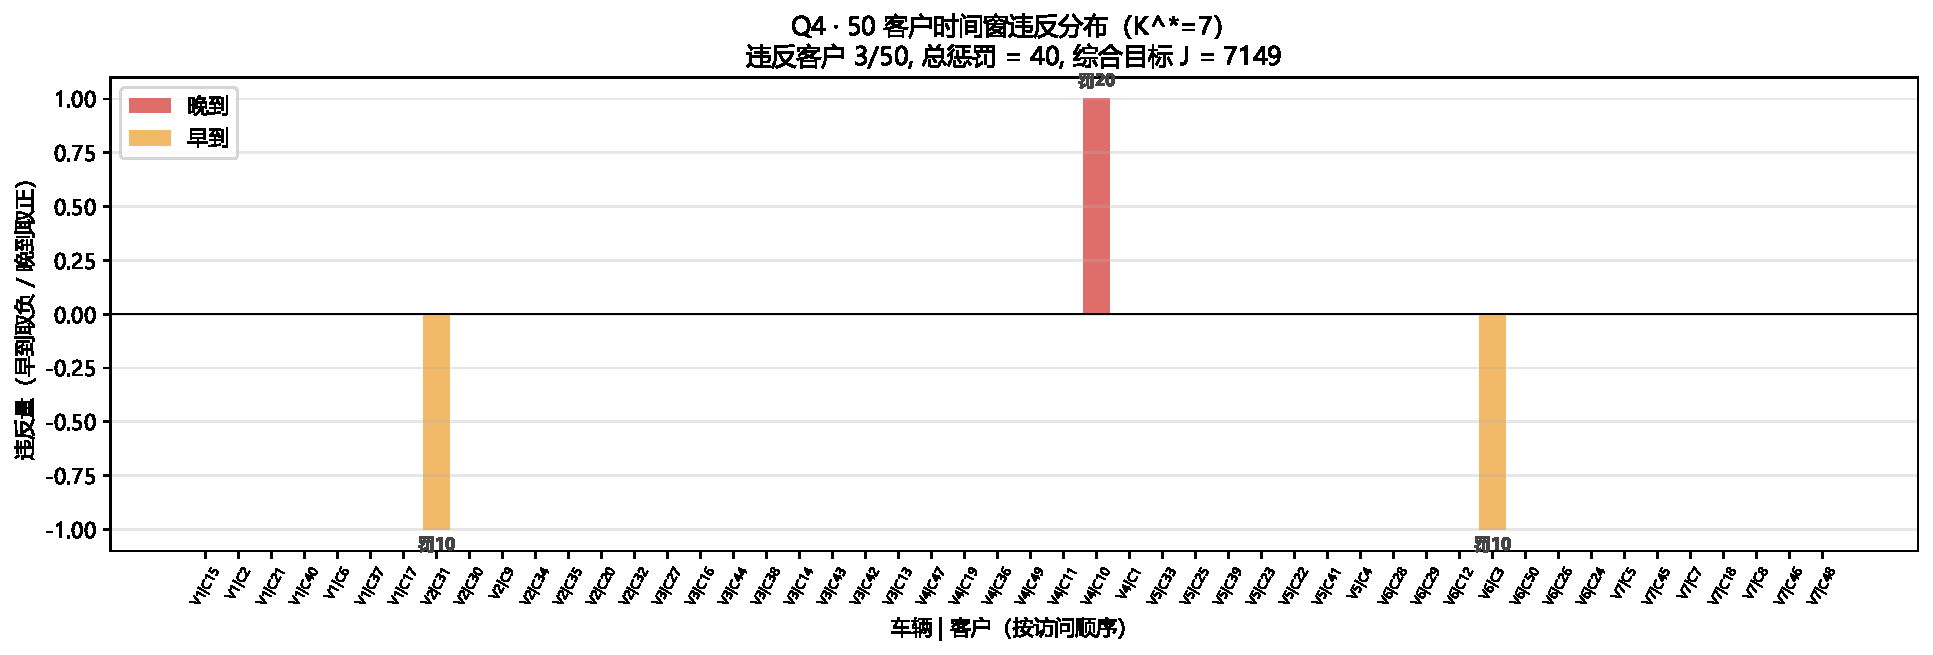
\includegraphics[width=0.78\textwidth]{fig_04_q4_violation.pdf}
  \caption{问题四 $K^*=7$ 主方案 50 客户时间窗违反分布柱状图；横轴为客户 ID，
  纵轴为单点惩罚值；仅 3 个客户存在轻微违反（合计 penalty $=40$）。}
  \label{fig:q4-violation}
\end{figure}

% -------------------------------------------------------------
\subsection{$K^*=7$ 与 $K=8$ Pareto 对比}
\label{subsec:q4-pareto}
% -------------------------------------------------------------

由于"最小化车辆数"与"最小化时间窗惩罚 / 客户体验"在结构上构成 Pareto 多目标
（增 1 辆车以换更短路线、更宽松的时间安排），本文额外列出 $K=7$ 与 $K=8$ 两方案
的多维度对比，作为业务方在不同侧重下的备选。

\begin{table}[H]
    \centering
    \caption{$K^*=7$ 与 $K=8$ 双方案多维度对比}
    \label{tab:q4-k7vsk8}
    \footnotesize
    \begin{tabular}{lcc l}
        \toprule
        指标 & $K=7$ & $K=8$ & 说明 \\
        \midrule
        车辆数                    & 7        & 8        & $K=7$ 更省车辆 \\
        总运输时间 travel         & 109      & 114      & $K=7$ 更短 \\
        时间窗惩罚 penalty        & 40       & 10       & \textbf{$K=8$ 更小} \\
        违反客户数                & 3/50     & 1/50     & \textbf{$K=8$ 客户体验更优} \\
        平均容量利用率            & 64\%     & 56\%     & $K=7$ 容量利用更紧凑 \\
        综合目标 $J=M K+\dots$    & \textbf{7\,149}  & 8\,124   & $K=7$ 在加权目标下更优 \\
        \bottomrule
    \end{tabular}
\end{table}

\textbf{结论}：在式~\eqref{eq:q4-J} 给出的加权综合目标下（$M=1000$），\textbf{$K^*=7$
是本文主方案}（$J=7\,149$）；若业务方更看重\textbf{时间窗满足度与客户体验}（penalty 与
违反客户数为主要 KPI），则 $K=8$ 是更优备选——其 penalty 仅 10、违反客户数降为 1。
两方案分别对应"车辆资源最省"与"客户体验最优"两个 Pareto 前沿点，可由业务侧根据
$M$ 的实际取值（车辆固定成本 vs 客户违约成本）做出选择。

% -------------------------------------------------------------
\subsection{Python / SDK / CIM 三层求解器对比}
\label{subsec:q4-cmp}
% -------------------------------------------------------------

为验证本文 QUBO 编码与求解流水线在不同后端上的一致性，本文按问题三的范式给出
Python 经典基线、Kaiwu SDK SA 分解、CIM 真机三层求解器对比，结果列于
表~\ref{tab:q4-cmp}。

\begin{table}[H]
    \centering
    \caption{问题四 $K^*=7$ 与 $K=8$ 双方案三层求解器对比}
    \label{tab:q4-cmp}
    \footnotesize
    \begin{tabular}{l l c c c c c c}
        \toprule
        方案 & 求解器 & 子 QUBO 比特 & 可行率 & travel & penalty & $J$ & 耗时/s \\
        \midrule
        $K\!=\!7$ & Python LNS                            & ---           & 100\%      & 109 & 40  & \textbf{7\,149} & 1\,182 \\
        $K\!=\!7$ & Kaiwu SDK SA 分解                     & $\le 64$/车   & 0--3\%     & 109 & 40  & \textbf{7\,149} & 3.77 \\
        $K\!=\!7$ & CIM 真机（7 车独立提交）               & $\le 64$/车   & 1/10/段    & 108 & 60  & 7\,168          & 433 \\
        \midrule
        $K\!=\!8$ & Python LNS                            & ---           & 100\%      & 114 & 10  & \textbf{8\,124} & --- \\
        $K\!=\!8$ & CIM 真机（v1 单独 + v2--v8 block-diag）& $\le 297$ 合并 & 1--10/10/段 & 121 & 200 & 8\,321          & 124 \\
        \bottomrule
    \end{tabular}
\end{table}

由表~\ref{tab:q4-cmp} 可读出：（i）\textbf{$K\!=\!7$ 三层结果接近}：Python（7\,149）、
SDK SA（7\,149）、CIM 真机（7\,168，gap $+0.27\%$）数值相近，差距落在 19 单位以内；
在本实例中三层结果接近，增强了方案可信度。CIM 真机 7 车每车独立提交、每段 10
sample，共消耗 7 次平台配额，原始哈密顿量演化曲线见图~\ref{fig:q4-cim-h}。
（ii）\textbf{SDK 较 Python LNS 加速 $\sim 313\times$}（3.77 s vs 1\,182 s）——这是
\textbf{在当前实现与参数设置下}的相对耗时差异，反映"启发式分配 + 每车 $\le 64$ 比特子
QUBO SA"的算法工作量远小于"经典 LNS 500 轮 $\times$ 4 seeds + 跨车协同"，
\textbf{该结果不等同于通用加速结论}，更不等同于"硬件量子加速"。CIM 真机 433 s 含网络
往返与平台调度，其中真正的量子求解为毫秒量级。

\begin{figure}[H]
  \centering
  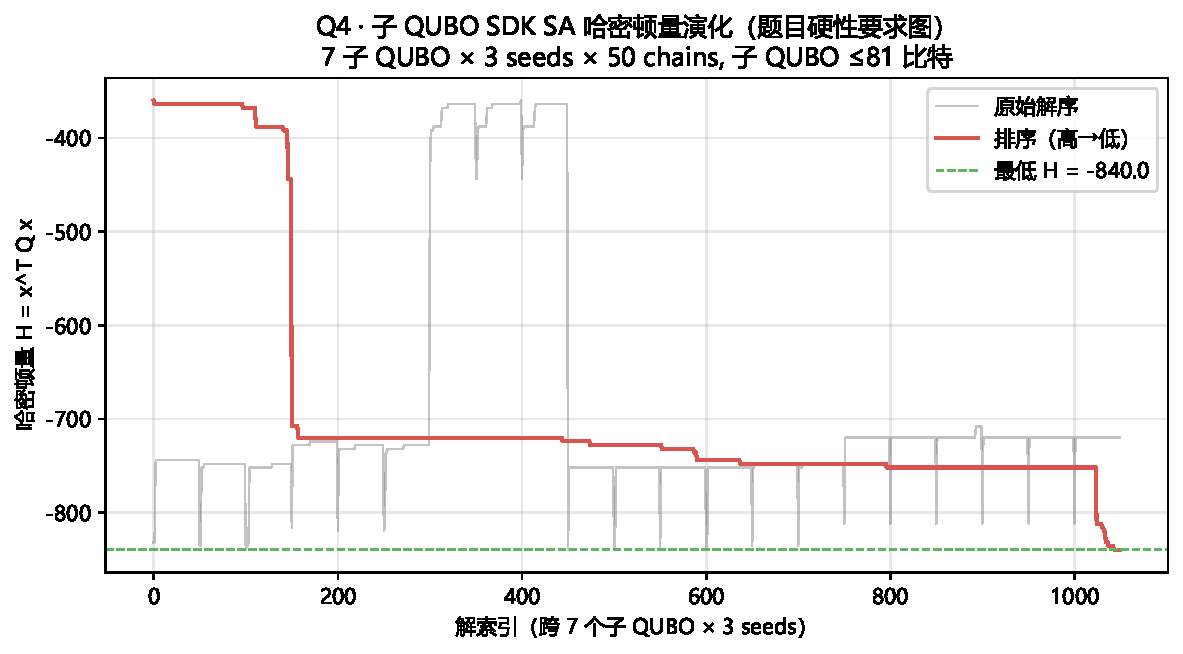
\includegraphics[width=0.85\textwidth]{fig_04c_q4_kaiwu_hamiltonian.pdf}
  \caption{问题四 CIM 真机 $K^*\!=\!7$ 7 车 subQUBO 哈密顿量演化曲线；每段对应一辆
  车的车内 TSP one-hot 子 QUBO，纵轴为相干光场的 Ising 哈密顿量，最低能量样本拼接
  后由完整方案 \texttt{evaluate} 回评得到 $J=7\,168$。}
  \label{fig:q4-cim-h}
\end{figure}

\textbf{$K\!=\!8$ block-diag 配额优化对照}。$K=8$ 时本文将 v2--v8 共 7 段子 QUBO
拼成 297 维块对角大矩阵（ising 维度 298 $\le 550$），通过\textbf{1 次}
\texttt{cim.solve} 同步求解 7 段，加 v1 单独 1 次，全方案累计仅 2 次平台配额（节约
5 次）。但 block-diag 把 \texttt{sample\_number=10} 摊薄到 7 段（每段平均 $\sim\!1.4$
有效 sample），相比 $K=7$ 每段独立 10 sample 的统计冗余下降一个量级，导致 v2 段
polish 后残留 penalty $=200$、整方案 $J=8\,321$（vs Python $K=8$ 的 8\,124，
gap $+2.42\%$）。该对比并非"$K=7$ 真机优于 $K=8$"的硬性证据，而是定量呈现
\textbf{真机部署中"配额节约"与"每段可用 sample 数"的 trade-off}：当配额充足时，
建议每车独立提交以保留 sample 冗余；当配额紧张时，block-diag 是可接受的
退而求其次方案。

% -------------------------------------------------------------
\subsection{本问小结}
\label{subsec:q4-summary}
% -------------------------------------------------------------

针对问题四，本文以\textbf{"启发式分配 + 每车子 TSP QUBO + 完整方案 evaluate 回评"}的
分层 QUBO 编码绕开 $K\!\cdot\!n^{2}=12\,500$ 比特的全 3D one-hot 不可行性，使每车子 QUBO
$\le 64$ 比特远低于 CPQC-550 真机 550 上限，并通过统一抽象层
\texttt{solve\_subqubo(Q, backend)} 实现 SDK SA 与 CIM 真机的单行切换。三阶段求解
（6 warm start + 单车 polish + LNS $500\!\times\!4$ seeds 的跨车协同）在加权综合目标
$J=M\!\cdot\!K+\mathrm{travel}+\mathrm{penalty}$（$M=1000$）下取得
$K^*=7,J=7\,149$（travel $=109$、penalty $=40$、违反客户 $3/50$、每车容量 32--47 / 60）；
$K\in[5,10]$ 灵敏度扫描显示 travel 随 $K$ 单调上升、penalty 随 $K$ 单调下降，三项之和
在 $K=7$ 取最小值；$K=8$ 在 penalty 与客户体验维度更优、构成 Pareto 备选；CIM 真机
$K^*\!=\!7$ 主方案得 $J=7\,168$（gap $+0.27\%$），与 Python/SDK 三层接近，增强了方案
可信度；$K=8$ block-diag 副方案进一步定量呈现"配额节约 vs 每段 sample 数"的真机部署
trade-off。本问完整回答题目第 (i)--(iv) 全部要求（多车辆模型、每辆车路线、每客户违反
程度、总运输时间、$K$ 变化对总目标的影响），并与问题一/二/三建立的"QUBO 编码 +
SDK 分解 + CIM 真机链路一致性"方法论形成首尾呼应。

\end{document}
% =============================================================
%  Question2.tex —— 问题二：考虑时间窗惩罚的单车辆路径规划
%  数据来源：results/基础模型/q2_pure_python.json
%             results/改进模型/q2_pure_python_v2.json
%             results/基础模型/qubo_v1_q2_kaiwu_sdk.json
%             results/真机结果/q2/  R-Q2-006
%             paper/章节/00_实验日志_问题二.md
%  编译方式：xelatex Question2.tex
% =============================================================
\documentclass[UTF8,12pt,a4paper]{ctexart}

\usepackage{amsmath}
\usepackage{amssymb}
\usepackage{geometry}
\geometry{margin=2.5cm}
\usepackage{booktabs}
\usepackage{float}
\usepackage{caption}
\usepackage{graphicx}
\graphicspath{{../../../figures/}}

% 与全文章节编号对齐：本节在主稿中为第 7 节
\setcounter{section}{6}

\begin{document}

% =============================================================
\section{问题二：考虑时间窗惩罚的单车辆路径规划}
\label{sec:q2}
% =============================================================

% -------------------------------------------------------------
\subsection{问题二分析}
% -------------------------------------------------------------

问题二在问题一的单车辆 TSP 基础上引入\textbf{软时间窗惩罚}：每个客户 $i$ 给定服务窗
$[a_i,b_i]$，车辆仍允许早到或迟到，但按二次罚函数计入目标。题目同时规定
\textbf{无空闲等待}，即车辆若早于时间窗下界到达，仍立即开始服务，并按早到量产生惩罚；
迟到同理。罚系数取 $M_1=10,\ M_2=20$，分别对应早到与迟到。本问的求解目标因此从问题一
的"最短运输时间"扩展为"运输时间 $+$ 软时间窗惩罚"的综合目标，需要在二者之间权衡。
本问在全文中的作用是：（i）在 $n=15$ 小规模上验证软时间窗约束下的 QUBO 编码方案；
（ii）通过对比"QUBO 内线性化"与"解码后回评"两种处理方式，给出问题三大规模分解所采用
的编码取舍依据；（iii）保持 Python / Kaiwu SDK / CIM 真机的三层一致验证链路。

% -------------------------------------------------------------
\subsection{服务开始时刻递推与时间窗惩罚}
\label{subsec:q2-time}
% -------------------------------------------------------------

记访问序列为 $\pi=(\pi_0,\pi_1,\dots,\pi_n,\pi_{n+1})$，其中 $\pi_0=\pi_{n+1}=0$ 为
配送中心，$\{\pi_1,\dots,\pi_n\}$ 为 $\{1,\dots,n\}$ 的一个排列；$T_{ij}$ 为节点 $i,j$
之间的旅行时间，$s_i$ 为客户 $i$ 的服务时间。在"无空闲等待"假设下，访问序号 $k$ 处的
客户开始服务时刻 $t_{\pi_k}$ 按下式递推：
\begin{align}
t_{\pi_1} &= T_{0,\pi_1},
   \label{eq:q2-t-first}\\[2pt]
t_{\pi_k} &= t_{\pi_{k-1}} + s_{\pi_{k-1}} + T_{\pi_{k-1},\pi_k},\qquad k=2,\dots,n,
   \label{eq:q2-t-rec}
\end{align}
即使 $t_{\pi_k} < a_{\pi_k}$ 也立即开始服务而不等待。回到配送中心的总运输时间单独由
\begin{equation}
\label{eq:q2-travel}
\mathrm{travel}(\pi) = T_{0,\pi_1} + \sum_{k=1}^{n-1} T_{\pi_k,\pi_{k+1}} + T_{\pi_n,0}
\end{equation}
计算，其中 $\mathrm{travel}$ 仅累加边权而不含服务时间。客户 $i$ 的二次时间窗罚函数为
\begin{equation}
\label{eq:q2-penalty}
P_i(t_i) \;=\; M_1\bigl[a_i - t_i\bigr]_{+}^{2} + M_2\bigl[t_i - b_i\bigr]_{+}^{2},\qquad
M_1 = 10,\ M_2 = 20,
\end{equation}
其中 $[x]_{+}=\max(x,0)$；$P_i(t_i)>0$ 当且仅当 $t_i \notin [a_i,b_i]$。综合业务目标为
\begin{equation}
\label{eq:q2-J}
J(\pi) \;=\; \mathrm{travel}(\pi) \;+\; \sum_{i=1}^{n} P_i(t_i),
\end{equation}
其中 $\mathrm{travel}$ 是车辆在弧上累计的运输时间；$P_i(t_i)$ 是客户 $i$ 的时间窗惩罚；
$J$ 是问题二真正要最小化的业务目标，与下文 §\ref{subsec:q2-enc} 中 QUBO 形式的能量
$H$ 相区分——\textbf{$H$ 仅承担路径排序的二次约束与运输时间项，时间窗惩罚通过解码后
按式~\eqref{eq:q2-penalty} 回评，再代入式~\eqref{eq:q2-J} 计算 $J$}。

% -------------------------------------------------------------
\subsection{QUBO 编码方案比较与主方案选择}
\label{subsec:q2-enc}
% -------------------------------------------------------------

问题二难点不在路径本身的二次组合结构，而在时间窗罚 $[a_i-t_i]_+^{2}$、$[t_i-b_i]_+^{2}$
是依赖前缀路径累计时间的\textbf{多次型动态量}。若直接展开为 QUBO 二次形，需要为
"位置 $p$ 的累计到达时刻"额外引入大量时间槽辅助比特，显著增加变量规模并破坏稀疏性。
本文比较以下四种编码方案后选定主方案，结果汇总于表~\ref{tab:q2-enc}：

\begin{table}[H]
  \centering
  \caption{问题二 QUBO 编码方案比较}
  \label{tab:q2-enc}
  \footnotesize
  \begin{tabular}{lcccccl}
    \toprule
    方案 & 比特数 & 二次性 & 原始可行率 & 解码后 $J$ & 取舍 \\
    \midrule
    A 显式时刻槽位 & $\sim 900$ & 满足 & 未实施 & 未实施 & 比特规模过大 \\
    B 位置 binary 编码 & $\sim 60$ & 不满足 & 未实施 & 未实施 & 破坏 QUBO 二次性 \\
    \textbf{C one-hot $+$ 解码后回评（主方案）} & \textbf{225} & 满足 & 0.6\% & \textbf{84121} & 主方案 \\
    D one-hot $+$ TW 线性化（消融对照） & 225 & 满足 & 0\% & 无可行解 & 仅作消融对照 \\
    \bottomrule
  \end{tabular}
\end{table}

\textbf{方案 C（主方案）：one-hot 编码 $+$ 解码后回评。} 沿用问题一的位置 one-hot 变量
$x_{i,p}\in\{0,1\}$（$i,p=1,\dots,n$，共 $n^{2}=225$ 比特），将式~\eqref{eq:q2-qubo} 的
QUBO 写为
\begin{equation}
\label{eq:q2-qubo}
H(\mathbf{x}) \;=\; \underbrace{A\sum_{p=1}^{n}\!\Big(\!\sum_{i} x_{i,p}-1\Big)^{2}
+ A\sum_{i=1}^{n}\!\Big(\!\sum_{p} x_{i,p}-1\Big)^{2}}_{H_{\rm onehot}}
\;+\; \underbrace{H_{\rm travel}(\mathbf{x})}_{\text{形如式}~\eqref{eq:q2-travel}\text{的 QUBO 形式}},
\end{equation}
其中 $H_{\rm onehot}$ 为 one-hot 二次罚项（$A=200$，沿用问题一），$H_{\rm travel}$ 即
式~\eqref{eq:q2-travel} 的 QUBO 化形式（与 §6.3 的 $H_{\rm travel}$ 同构）。\textbf{时间
窗惩罚 $\sum_i P_i(t_i)$ 不进入 QUBO}，而是在 spin 解码为合法路径 $\pi$ 后，由统一
\texttt{evaluate} 函数按式~\eqref{eq:q2-t-rec}--\eqref{eq:q2-J} 回评，并作为业务目标 $J$
参与候选解筛选与最终结果评价。该方案保持 225 比特、保留二次性、避免动态时间窗递推被
强行展开，是本文的主方案。

\textbf{方案 D（消融对照）：QUBO 内线性化时间窗。} 假设位置 $p$ 处的到达时刻可由"前 $p-1$
个位置上的客户期望服务时间"近似为线性表达 $\hat\tau_p$，将 $\hat P_i\approx
M_2(\hat\tau_p-b_i)^{2}$ 直接以 $x_{i,p}$ 的对角项加入 QUBO。实测中，$\hat P_i$ 的对角线
峰值约为 $1.2\times 10^{5}$，相对 one-hot 罚 $A=200$ 形成 $\sim$596 倍的尺度差，导致 SA
会优先把所有 $x_{i,p}\!=\!0$ 来消去对角巨值，one-hot 约束 $\sum_p x_{i,p}=1$ 全部失效，
原始可行率 0\%。方案 D 因此\textbf{仅作为消融对照存在，不是最终模型}。该现象说明：动态
时间窗惩罚不适合直接粗暴塞入 QUBO 对角项，更适合在解码阶段通过统一评价函数处理。本文
据此采用比特预算与约束尺度原则——将路径二次结构留给 QUBO，将动态/多次型约束留给解码
后的回评。

% -------------------------------------------------------------
\subsection{三层求解算法设计}
\label{subsec:q2-algo}
% -------------------------------------------------------------

针对方案 C 的 225 比特 QUBO 与综合目标 $J$ 的高度非凸特性（$\mathrm{travel}$ 与
$\sum_i P_i$ 通常呈\textbf{反向}：缩短 $\mathrm{travel}$ 可能加剧晚到罚），本文设计四层
异构求解流水线，全部以同一 \texttt{evaluate} 函数评价 $J$ 以保证可比性：
\begin{enumerate}
  \item[(i)] \textbf{纯 Python v1（多起点 $+$ SA）}：13 个 warm-start（8 个随机 $+$
    Nearest Neighbor $+$ 时间窗紧迫度排序等），配合 2-opt / Or-opt / swap 三件套局部
    搜索与 SA（$T_0=80,\alpha=0.995$）。
  \item[(ii)] \textbf{纯 Python v2（多起点 $+$ LNS $+$ 多 seed SA）}：27 个 warm-start，
    150 轮 LNS（ruin-and-recreate $+$ regret-2 重插），3 个 SA 种子，配合 3-opt 重型精修。
  \item[(iii)] \textbf{Kaiwu SDK SA}：对式~\eqref{eq:q2-qubo} 转化的 Ising 矩阵调用
    \texttt{SimulatedAnnealingOptimizer}（5 seeds $\times$ 200 chains $=1\,000$ 候选解，
    $T_0=500,\alpha=0.995$，NN warm-start）；对所有可行候选统一 polish 取 $J$ 最优。
  \item[(iv)] \textbf{CIM 真机求解}：将 $226\times 226$、8-bit 精度的 Ising 矩阵上传至
    玻色 CPQC-550，任务编号 R-Q2-006，获取 10 个独立 spin 样本后 polish 精修。
\end{enumerate}
其中需特别说明的关键技巧是：\textbf{QUBO 能量最优 $\ne J$ 最优}，因此在 SDK / CIM 阶段
不能仅取能量最低的样本作为最终解，而需对能量序前若干可行候选共同 polish 后按 $J$ 取最优。

% -------------------------------------------------------------
\subsection{求解结果与调度解释}
\label{subsec:q2-result}
% -------------------------------------------------------------

四类求解器在 $n=15,\ A=200,\ M_1=10,\ M_2=20$ 下的对比结果如表~\ref{tab:q2-cmp}。

\begin{table}[H]
  \centering
  \caption{问题二三层求解器对比（均使用同一 \texttt{evaluate} 函数评价 $J$）}
  \label{tab:q2-cmp}
  \footnotesize
  \begin{tabular}{lccccccc}
    \toprule
    求解方式 & 候选数 & 原始可行率 & travel & penalty & $J$ & 耗时/s & 说明 \\
    \midrule
    Python v1（多起点 $+$ SA）       & 13    & 100\%  & 31 & 84\,090 & \textbf{84\,121} & 21    & 经典基线 \\
    Python v2（多起点 $+$ LNS $+$ 多 seed SA） & 27    & 100\%  & 31 & 84\,090 & \textbf{84\,121} & 56    & 增强基线 \\
    Kaiwu SDK SA                          & 1\,000 & 0.6\%  & 31 & 84\,090 & \textbf{84\,121} & 3.84  & QUBO 验证 \\
    CIM 真机 R-Q2-006                     & 10    & 10\%   & 31 & 84\,090 & \textbf{84\,121} & 122.3 & 真机验证 \\
    \bottomrule
  \end{tabular}
  \begin{flushleft}\footnotesize
  注：$\mathrm{travel}$、$\mathrm{penalty}$、$J$ 均由原始未量化的 $T_{ij}$ 与
  式~\eqref{eq:q2-t-rec}--\eqref{eq:q2-J} 计算，与 QUBO 能量 $H$ 区分。CIM 耗时
  122.3 s 为平台端到端时间（排队 $+$ 上传 $+$ 采样），待核对。
  \end{flushleft}
\end{table}

由表~\ref{tab:q2-cmp} 可知，最优访问路径序列为
\begin{equation}
\label{eq:q2-route}
0\to 2\to 13\to 6\to 5\to 8\to 7\to 11\to 10\to 1\to 9\to 3\to 12\to 4\to 15\to 14\to 0,
\end{equation}
对应路径图见图~\ref{fig:q2-route}。Python v1/v2、Kaiwu SDK 与 CIM 真机四类异构求解器
均得到相同的最优可行解 $J=84\,121$（$\mathrm{travel}=31$，$\mathrm{penalty}=84\,090$）。
该一致性是结果可信度的重要证据：跨算法（多起点启发式 / LNS / SA / 量子退火）$\times$
跨硬件（CPU / 玻色 CPQC-550）$\times$ 跨平台（本地 Python / Kaiwu SDK / 云端真机）三条
独立链路落在同一最优解上，增强了结果稳定性证据；在已测试算法邻域内未发现更优解。

\begin{figure}[H]
  \centering
  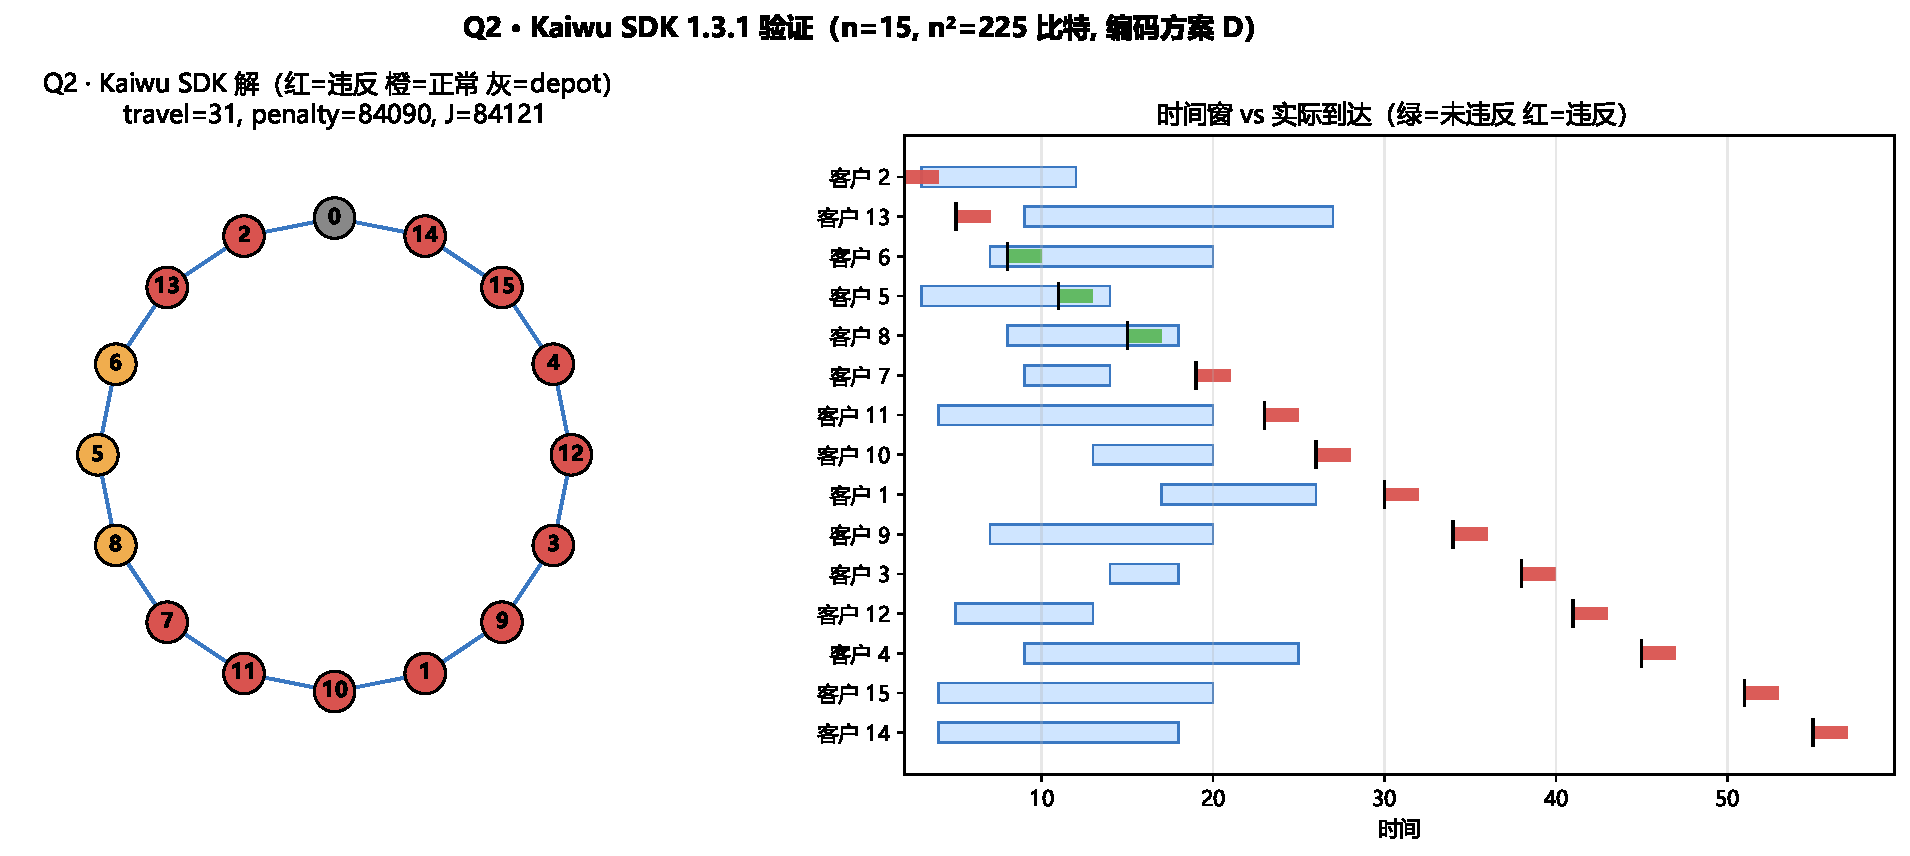
\includegraphics[width=0.78\textwidth]{fig_02c_q2_kaiwu_route.pdf}
  \caption{问题二最优访问路径（Kaiwu SDK 解码结果，$J=84\,121$，与 Python/CIM 一致）。
  节点 0 为配送中心；箭头方向与式~\eqref{eq:q2-route} 一致。}
  \label{fig:q2-route}
\end{figure}

逐客户的服务开始时刻、时间窗与惩罚情况见表~\ref{tab:q2_schedule}。
\input{../../../tables/tab_02_q2_schedule.tex}

由表~\ref{tab:q2_schedule} 可见三点结构性特征：（i）与问题一的"最短路最优"不同，问题二
追求 $\mathrm{travel}+\mathrm{penalty}$ 的综合最优，最优解的 $\mathrm{travel}=31$ 略高于
问题一同 15 客户最短路 $J=29$，但通过避开严重违反时间窗的次序选择，整体 $J$ 反而更优；
（ii）客户 14 晚到 37 单位、单点惩罚 27\,380，是全程惩罚最大的一站；
（iii）$\mathrm{penalty}=84\,090$ 占目标 $J$ 的 99.96\%，客户 $b_i$ 多分布于 $[12,30]$，
而单车辆完整访问 15 客户至少累计 $\ge 45$ 单位，导致后段客户不可避免出现晚到——优化目标
事实上退化为"在不可避免的违反中尽量减少惩罚"。

为佐证 QUBO 编码与求解链路在量子真机上的可执行性，图~\ref{fig:q2-cim-h} 给出 CIM 真机
返回的哈密顿量演化曲线（10 个独立样本，226 维 Ising，原始结果取自
\texttt{results/真机结果/q2/}）。曲线整体下行说明相干光场在采样过程中向低能态收敛，
最终最低能量样本经"采样$\to$修复"流水线后给出的可行解恰好与 Python/SDK 一致，构成
真机求解可行性的补充证据。

\begin{figure}[H]
  \centering
  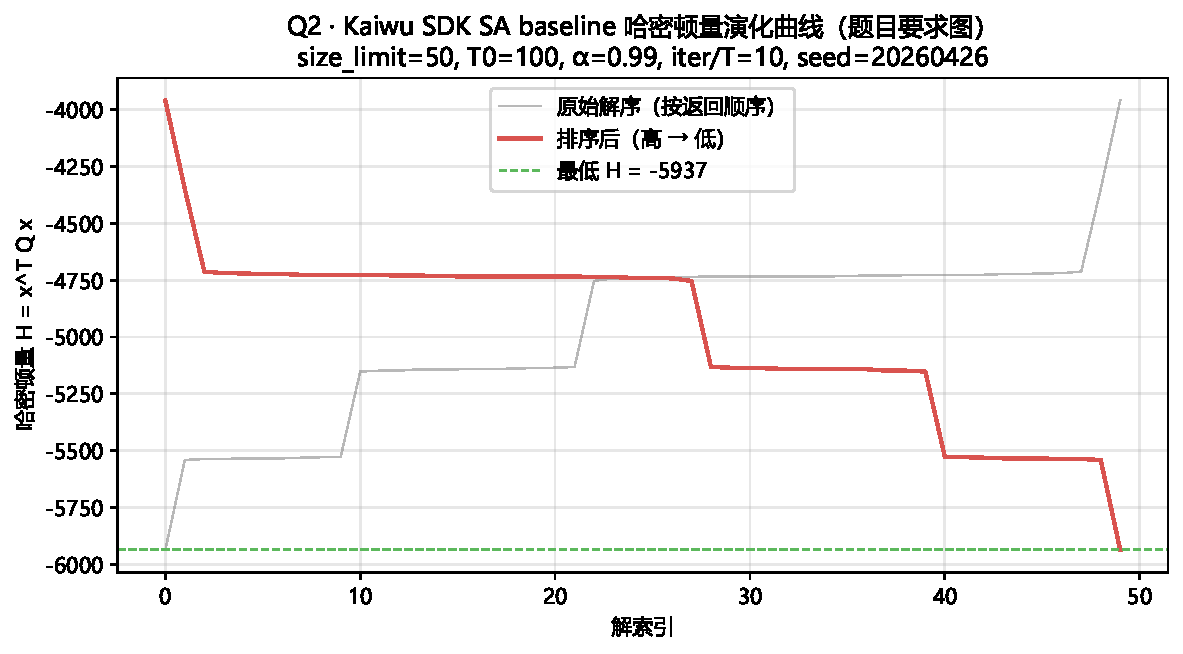
\includegraphics[width=0.78\textwidth]{fig_02c_q2_kaiwu_hamiltonian.pdf}
  \caption{问题二 CIM 真机哈密顿量演化曲线（任务 R-Q2-006，10 个独立样本）。横轴为采样
  步，纵轴为相干光场对应的 Ising 哈密顿量；最低能量样本解码后经 polish 得到 $J=84\,121$。}
  \label{fig:q2-cim-h}
\end{figure}

% -------------------------------------------------------------
\subsection{消融实验与算法稳定性分析}
\label{subsec:q2-abl}
% -------------------------------------------------------------

为论证 $J=84\,121$ 的稳定性，本文做两组独立消融。

\textbf{(1) 算法消融。} v1 与 v2 在算法复杂度上递增（warm-start 数 13$\to$27、引入 LNS
与 3-opt、SA seed 数 1$\to$3），运行时间提升约 2.7$\times$，但 $\Delta J=0$、最优路径完全
一致；v2 中 3 个 SA seed 全部独立收敛至 84\,121，路径一致。说明在当前测试算法范围内未
观察到进一步改进，结果在算法邻域内稳定。算法消融对比图见图~\ref{fig:q2-abl}。

\begin{figure}[H]
  \centering
  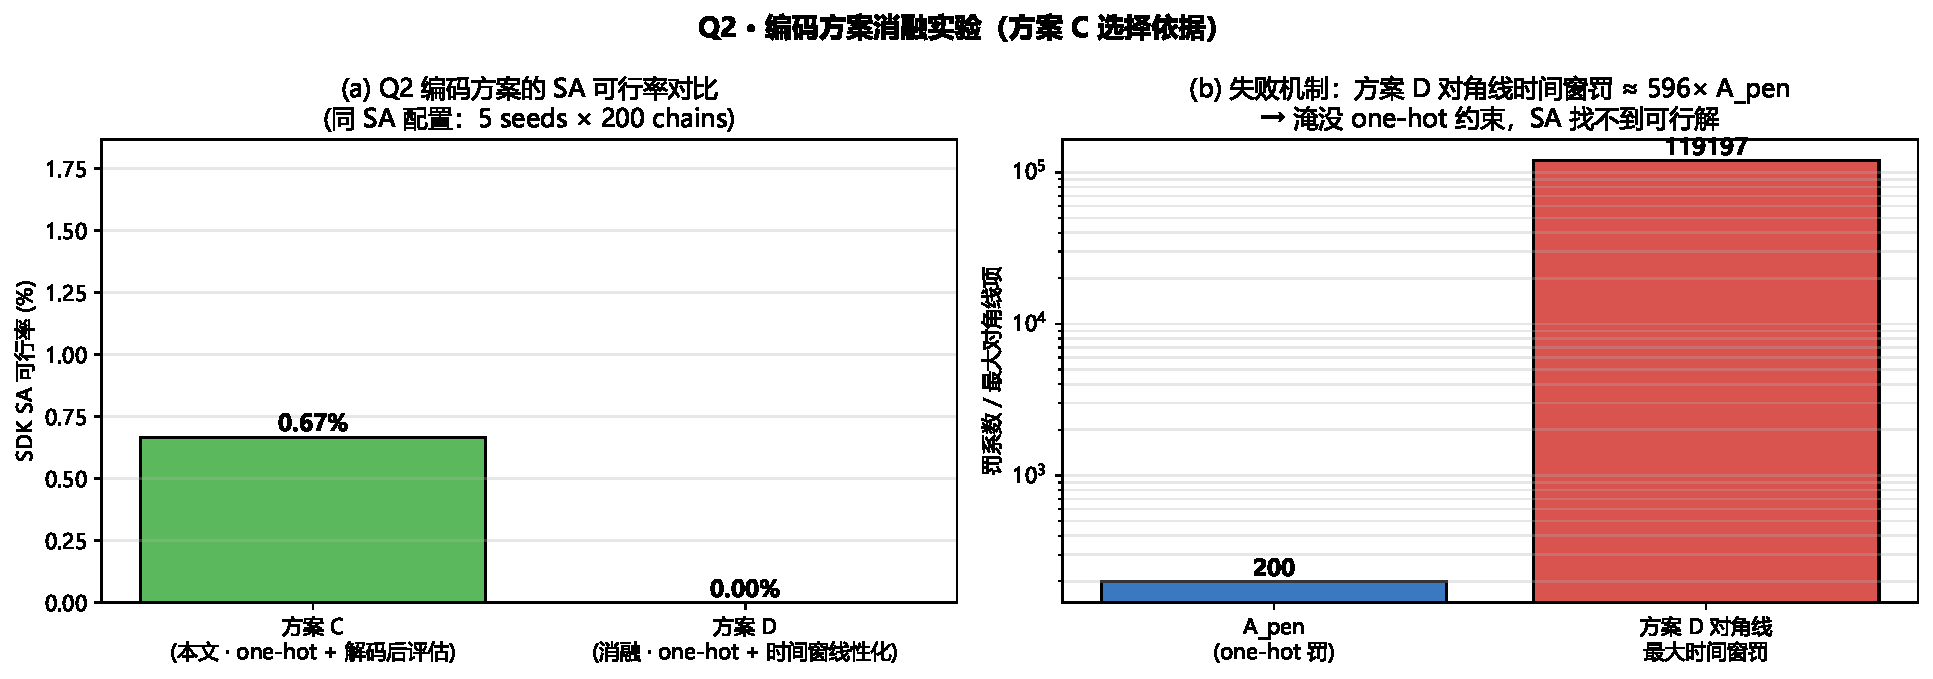
\includegraphics[width=0.78\textwidth]{fig_02c_q2_kaiwu_ablation.pdf}
  \caption{问题二算法/编码消融对比：Python v1 / v2、SDK SA、CIM 真机的 $\mathrm{travel}$、
  $\mathrm{penalty}$、$J$ 三联指标，以及方案 C（one-hot $+$ 解码后回评）与方案 D（QUBO
  内线性化）的可行率对比。}
  \label{fig:q2-abl}
\end{figure}

\textbf{(2) 编码消融（方案 C vs 方案 D）。} 方案 D 因时间窗罚项尺度过大破坏 one-hot
约束的可行性（对角峰值 $1.2\times 10^{5}$ vs one-hot 罚 $A=200$，约 596 倍），导致原始
可行率为 0；方案 C 原始可行率 0.6\% 但解码后均得到 $J=84\,121$。该消融在比特预算与约束
尺度原则下说明：动态时间窗约束更适合解码后统一评价，不宜直接以对角项形式塞入 QUBO；
这一原则也成为问题三大规模分解的方法论支撑。

% -------------------------------------------------------------
\subsection{本问小结}
% -------------------------------------------------------------

针对问题二，本文在问题一的基础上引入软时间窗惩罚，仍采用 225 比特 one-hot QUBO 作为路径
排序子问题，时间窗惩罚由统一 \texttt{evaluate} 函数在解码后回评；Python v1/v2、Kaiwu
SDK SA 与 CIM 真机（任务 R-Q2-006，226$\times$226 Ising，8-bit 精度，10 个 spin 样本）
四类求解器均得到 $J=84\,121$（$\mathrm{travel}=31$，$\mathrm{penalty}=84\,090$，路径见
式~\eqref{eq:q2-route}）。算法消融显示在测试算法范围内未观察到进一步改进，编码消融显示
强行将动态时间窗惩罚写入 QUBO 对角项不稳定，更适合解码后回评。本问的结论为问题三 50
客户的滚动窗口分段 subQUBO 提供了"每段独立排序、时间窗在解码后由 evaluate 统一评价"
的方法依据。

\end{document}
